%\documentclass[12pt,a4paper,faculty=we,language=nl]{ugent-doc}
%
%% Optional: margins and spacing
%%-------------------------------
%% Uncomment and adjust to change the default values set by the template
%% Note: the defaults are suggested values by Ghent University
%\geometry{bottom=2.5cm,top=2.5cm,left=2.5cm,right=2.5cm}
%%\renewcommand{\baselinestretch}{1.15} % line spacing
%
%
%% Font
%%------
%\usepackage[T1]{fontenc}
%\usepackage[utf8]{inputenc}
%% Comment/remove the two lines below to use the default Computer Modern font
%\usepackage{libertine}
%\usepackage{libertinust1math}

% Proper word splitting
%-----------------------
%\usepackage[dutch]{babel}

% Mathematics
%-------------

\documentclass[11pt,dutch,faculty=we,layout=titlefont,underline=false,titleUppercase=true,titleUnderline=true]{ugent2016-report}
\usepackage[dutch]{babel}
\usepackage{fontspec,unicode-math}
\usepackage{amsmath}
\usepackage{subcaption}
\usepackage{csquotes}
\usepackage{subfloat}
\usepackage{float}

% Figures
%---------
\usepackage{graphicx, ugent2016-assets}
\graphicspath{{./figures/}}
\usepackage{hyperref}
\hypersetup{
    colorlinks,
    linkcolor={black},
    citecolor={blue!50!black},
    urlcolor={blue!80!black}
}
\usepackage{booktabs,makecell}

\setlength{\parindent}{0em}

\author{Bram Devlaminck}
\title{Unipept:\newline geavanceerde indexstructuren \newline voor identificatie en analyse\newline van arbitraire peptiden}
%\subtitle{Hello}
\academicyear{2023--2024}
\programme{Informatica}
\studentnumber{01902993}
\email{bram.devlaminck@ugent.be}
\promotors{Prof.\ Dr.\ Peter Dawyndt\newline Prof.\ Dr.\ Bart Mesuere}

% Bibliography settings
%-----------------------
\usepackage[
%    backend=biber,
%    maxcitenames=1,
%    maxbibnames=2,
%    hyperref=true
]{biblatex}
\addbibresource{bibliography.bib}
%\addbibresource{./bibliography.bib}
% \usepackage{csquotes} % Suggested when using babel+biblatex
% local run procedure: (1) pdfLatex on main, (2) biber on main, (3) pdfLatex on main, (4) pdfLatex on main

% Hyperreferences
%-----------------
%\usepackage[colorlinks=true, allcolors=ugentblue]{hyperref}

% Whitespace between paragraphs and no indentation
%--------------------------------------------------
%\usepackage[parfill]{parskip}

% Input for title page
%----------------------

%% The title
%\thetitle{\color{ugentblue}Unipept:\newline geavanceerde indexstructuren \newline voor identificatie en analyse\newline van arbitraire peptiden}
%\thesubtitle{\color{black}Bram Devlaminck} % Optional

%% Note: a stricter UGent style could be achieved with, e.g.:
%\usepackage{ulem}
%\renewcommand{\ULthickness}{2pt}
%\thetitle{\uline{\color{ugentblue}INCLASS KAGGLE COMPETITION:\newline LOAN-DEFAULT PREDICTION}}
%% Note: do not forget to reset the \ULthickness to 1pt after invoking \maketitle
%\renewcommand{\ULthickness}{1pt}

%% The first (top) infobox at bottom of titlepage
%\infoboxa{\bfseries\large Masterproef}
%
%
%% The second infobox at bottom of titlepage
%\infoboxb{Promotoren:
%    \begin{tabular}[t]{l}
%        Prof.\ Dr.\ Peter Dawyndt \\ % note syntax 'short space'
%        Prof.\ Dr.\ Bart Mesuere
%    \end{tabular}
%}
%
%% The third infobox at bottom of titlepage
%\infoboxc{Begeleiders:
%    \begin{tabular}[t]{l}
%        Pieter Verschaffelt \\ % note syntax 'short space'
%        Tibo Vande Moortele
%    \end{tabular}
%}
%
%% The last (bottom) infobox at bottom of titlepage
%\infoboxd{Academisch jaar: 2023--2024} % note dash, not hyphen


\begin{document}

    \maketitle


    \setmonofont[Scale=MatchLowercase,Contextuals={Alternate}]{Jetbrains Mono}
% =====================================================================
% Cover
% =====================================================================

    \chapter*{Toelating tot bruikleen}

De auteur geeft de toelating deze masterproef voor consultatie beschikbaar te stellen en delen van de masterproef te kopiëren voor persoonlijk gebruik.
Elk ander gebruik valt onder de bepalingen van het auteursrecht, in het bijzonder met betrekking tot de verplichting de bron uitdrukkelijk te vermelden bij het aanhalen van resultaten uit deze masterproef.
\\ \\
Bram Devlaminck \\ \today


% =====================================================================
% Front matter
% =====================================================================

% ------------ TABLE OF CONTENTS ---------
    \tableofcontents
    \newpage


% =====================================================================
% Main matter
% =====================================================================


    \chapter{Introductie}\label{sec:introductie}


    \section{Probleemstelling}
    Unipept is een toolset die vooral gericht is op de analyse van stalen uit in het onderzoeksveld van de metaproteomica.
    Om uit te leggen wat metaproteomica is, is het nuttig eerst te weten wat de discipline van proteomica onderzoekt.
    In proteomica wordt een set van proteïnen komende uit 1 organism onderzocht om daaruit informatie te halen.
    Het prefix meta uit metaproteomica slaat op het feit dat in deze discipline stalen onderzocht worden waarin de proteïnen van meerdere organismen (meestal uit dezelfde biologische omgeving) voorkomen.
    Dit maakt de analyse moeilijker aangezien proteïnen van verschillende organismen gelijkaardige amino zuur sequenties kunnen hebben (al dan niet puur door toeval).
    \\ \\
    Op dit moment is Unipept gericht op de analyse van tryptische peptiden.
    Dit zijn peptiden die ontstaan na het knippen van proteïnen aan de hand van trypsine.
    Dit is een protease (eiwitafbrekend enzym) dat proteïnen opsplitst in meerdere peptiden.
    Er zijn nog andere proteases die gebruikt kunnen worden, maar trypsine is de meeste gebruikte aangezien het de proteïnen op vaste plaatsen knipt.
    \\ \\
    Trypsine zal een eiwit knippen na elke voor komen van lysine (K) or arginine (R) indien het opeenvolgende aminozuur geen proline (P) is
    Deze vuistregel is echter niet perfect.
    Soms zal trypsine echter een locatie waar normaal geknipt zou worden missen.
    Dit wordt dan een \textit{missed cleavage} genoemd.
    \\ \\
    Deze peptiden worden dan daan de hand van een massa spectrometer gewogen (TODO: wat wordt hier mee gedaan?) en na een ingewikkeld zoekproces (via zogenaamde zoekmachines) omgezet naar een string die de peptide sequentie voorstelt.
    Deze peptide sequenties zijn de input voor Unipept.
    \\ \\
    Zoals eerder vermeld, is Unipept een tool die specifiek gericht is op het analyseren van tryptische peptiden.
    De reden hiervoor is de manier waarop de achterliggende index-structuur die Unipept gebruikt opgebouwd wordt.
    In gaat als volgt in grote lijnen:
    \begin{enumerate}
        \item Haal alle proteïnen op uit de UniProtKB databank.
        \item Splits deze proteïnen volgens de vuistregel die trypsine volgt.
        \item Sla alle resulterende tryptische peptiden op in een index-structuur.
    \end{enumerate}
    \leavevmode\newline
    Als voordeel heeft dat dit toelaat efficiënt tryptische peptiden te zoeken.
    Er is echter een belangrijke keerzijde aan deze manier van werken:
    \begin{enumerate}
        \item Niet-tryptische peptiden (die bv gesplitst zijn aan de hand van een ander protease) kunnen niet gezocht worden.
        \item Tryptische peptiden met \textit{missed cleavage} zijn inefficiënt om te zoeken omdat tijdens het opbouwen van de Unipept index-structuur de vuist regel gevolgd wordt, en er dus nooit gemiste knippen zijn.
    \end{enumerate}
    Op dit moment is er voor het 2e puntje wel een work-around die toe laat deze peptiden toch te zoeken (maar met een erg significante performantie overhead).
    Dit verklaart dan ook de nood voor een nieuwe index-structuur die deze 2 tekortkomingen op lost.
    Dit is exact waar deze thesis op focust.
    \newline
    Voor een gedetailleerdere beschrijving over Unipept en het onderzoeksveld van metaproteomica raad ik aan om de inleiding van het doctoraat van Dr. Pieter Verschaffelt (TODO: is pieter dokter?) te lezen.
    Deze inleiding is dan ook gebaseerd daarop~\cite{phdPieterUnipept}.


    \section{Test Datasets}\label{sec:datasets}

    \subsection{Proteïne databanken}
    Om te testen hoe goed een implementatie is en hoe deze vergelijkt met al bestaande implementaties is het belangrijk om enkele representatieve datasets te hebben.
    De gebruikte datasets zijn allemaal eiwit databanken die een subset zijn van UniProt (meer specifiek UniProtKB 2023\_04) (TODO: cite uniprot).
    UniprotKB is een eiwit databank die in 2 grote delen op te splitsen valt.
    \begin{enumerate}
        \item Swiss-Prot: Dit is een kleinere, manueel gecureerde, dataset die 570 157 eiwit sequenties bevat.
        \item TrEMBL: Deze dataset bevat 251 600 768 sequenties en is dus veel groter dan Swiss-Prot.
        Het grote verschil is dat deze dataset \textbf{niet} manueel gecureerd is.
    \end{enumerate}

    Om het benchmarken van implementaties praktisch te houden maak ik gebruik van 2 Subsets hiervan.

    \paragraph{Swiss-Prot} Dit is de standaard Swiss-Prot databank die deel is van UniProt (zoals eerder uitgelegd).
    Een kort overzicht van alle statistieken is terug te vinden in tabel~\ref{tab:swissprot_eigenschappen} terwijl figuur~\ref{fig:swissprot_aminozuur} en figuur~\ref{fig:swissprot_length} meer inzicht geven in de distributie van de aminozuren en lengte van de proteïnen.

    \begin{table}[h!]
        \centering
        \begin{tabular}{c c}
            Metriek                    & Waarde      \\
            \hline\hline
            Totaal aantal sequenties   & 569 619     \\
            Totale lengte              & 205 954 074 \\
            Minimale proteïne lengte   & 2           \\
            Maximale proteïne lengte   & 35 213      \\
            Gemiddelde proteïne lengte & 361.56      \\
            Mediaan proteïne lengte    & 295         \\
            \hline
        \end{tabular}
        \caption{Eigenschappen van de Swiss-Prot databank}
        \label{tab:swissprot_eigenschappen}
    \end{table}


    \begin{figure}[H]
        \centering
        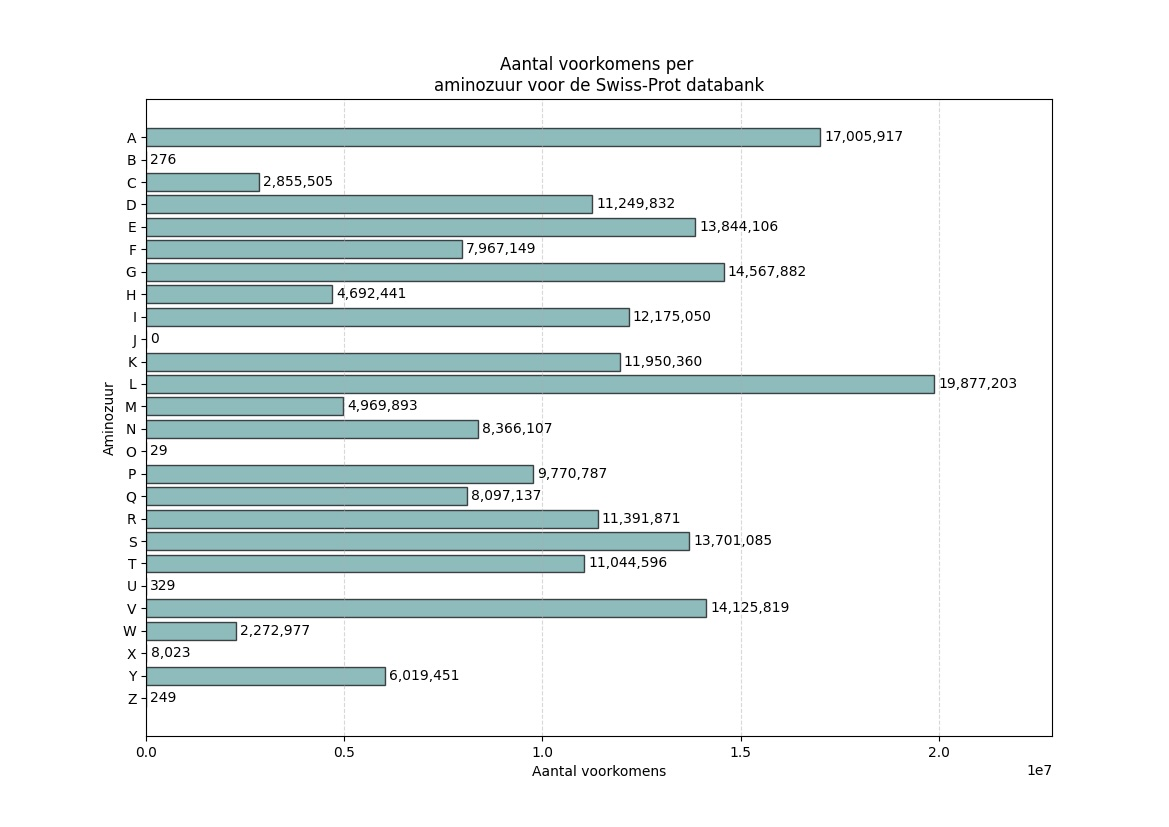
\includegraphics[width=0.7\linewidth]{swissprot_aminozuur_voorkomens}
        \caption{Aantal voorkomens per aminozuur voor alle proteïnen in de Swiss-Prot databank}
        \label{fig:swissprot_aminozuur}
    \end{figure}

    \begin{figure}[H]
        \centering
        \subfloat[Overzicht van lengte distributie alle proteïnen]{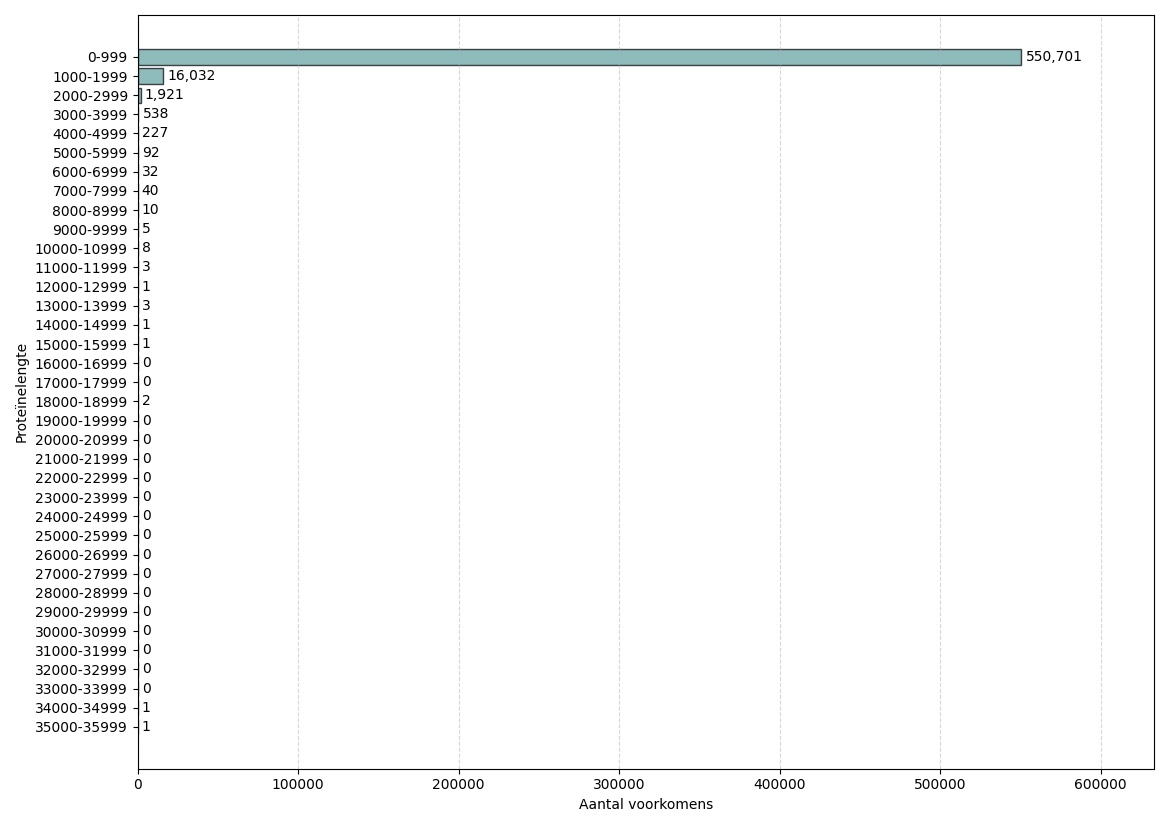
\includegraphics[width=0.5\linewidth]{swissprot_length_distribution_large}}
        \subfloat[Ingezoomd beeld van de lengtedistributie tot 1000 aminozuren lang]{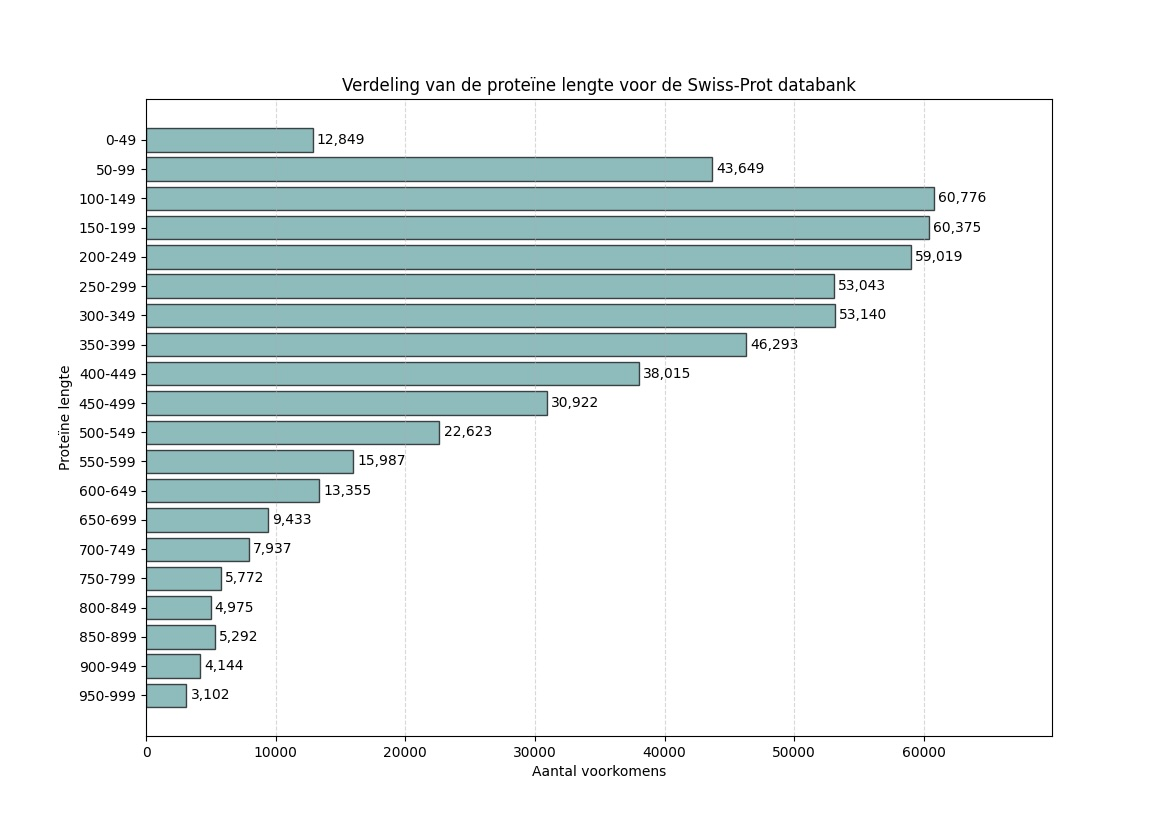
\includegraphics[width=0.5\linewidth]{swissprot_length_distribution_small}}
        \caption{Lengtedistributie van de proteïnen in de Swiss-Prot databank}\label{fig:swissprot_length}
    \end{figure}

    Een klein detail dat valt op te merken is dat in tabel \ref{tab:swissprot_eigenschappen} het totaal aantal sequenties iets kleiner is dan wat eerder aangegeven is.
    Dit is omdat het gebruikte input bestand een voorwerkt bestand is dat al door een deel van de Unipept pipeline verwerkt is.
    Hierbij worden sequenties met een taxon id dat niet in de Unipept databank zit verwijderd.
    Dit verklaart het kleine verschil.

    \paragraph{Human-Prot} Deze dataset is samengesteld aan de hand van 3 referentiedatabanken die deel uit maken van UniProt.
    Deze werd geleverd aan me door mijn begeleider Pieter Verschaffelt.
    \begin{enumerate}
        \item Human Genome~\cite{proteomes_homo_sapiens}
        \item Influenza B~\cite{proteomes_infuenza_b}
        \item Human Papillomavirus~\cite{proteomes_human_papillomavirus}
    \end{enumerate}

    Deze Human-Prot databank is nog kleiner dan Swiss-Prot wat het testen tijdens ontwikkeling sneller maakt.
    In tabel~\ref{tab:humanprot_eigenschappen} valt een korte samenvatting te zien van enkele kenmerken van deze dataset.
    Opnieuw is er in figuur~\ref{fig:humanprot_aminozuur} en figuur~\ref{fig:humanprot_length} een gedetailleerder overzicht te vinden.

    \begin{table}[h!]
        \centering
        \begin{tabular}{ c c }
            Metriek                    & Waarde     \\
            \hline\hline
            Totaal aantal sequenties   & 82 695     \\
            Totale lengte              & 30 293 046 \\
            Minimale proteïne lengte   & 2          \\
            Maximale proteïne lengte   & 35 991     \\
            Gemiddelde proteïne lengte & 366.32     \\
            Mediaan proteïne lengte    & 204        \\
            \hline
        \end{tabular}
        \caption{Eigenschappen van de Human-Prot databank}
        \label{tab:humanprot_eigenschappen}
    \end{table}

    \begin{figure}[H]
        \centering
        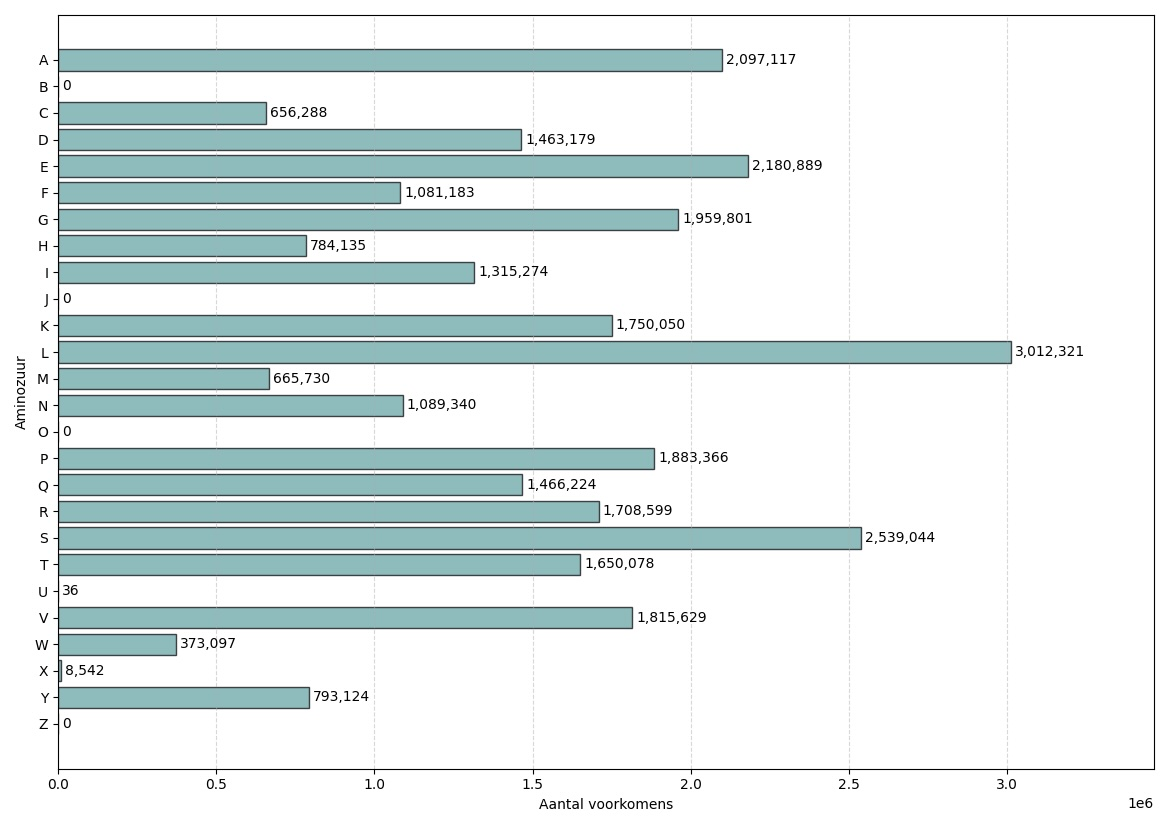
\includegraphics[width=0.7\linewidth]{humanprot_aminozuur_voorkomens}
        \caption{Aantal voorkomens per aminozuur voor alle proteïnen in de Human-Prot databank}
        \label{fig:humanprot_aminozuur}
    \end{figure}

    \begin{figure}[H]
        \centering
        \subfloat[Overzicht van lengte distributie alle proteïnen]{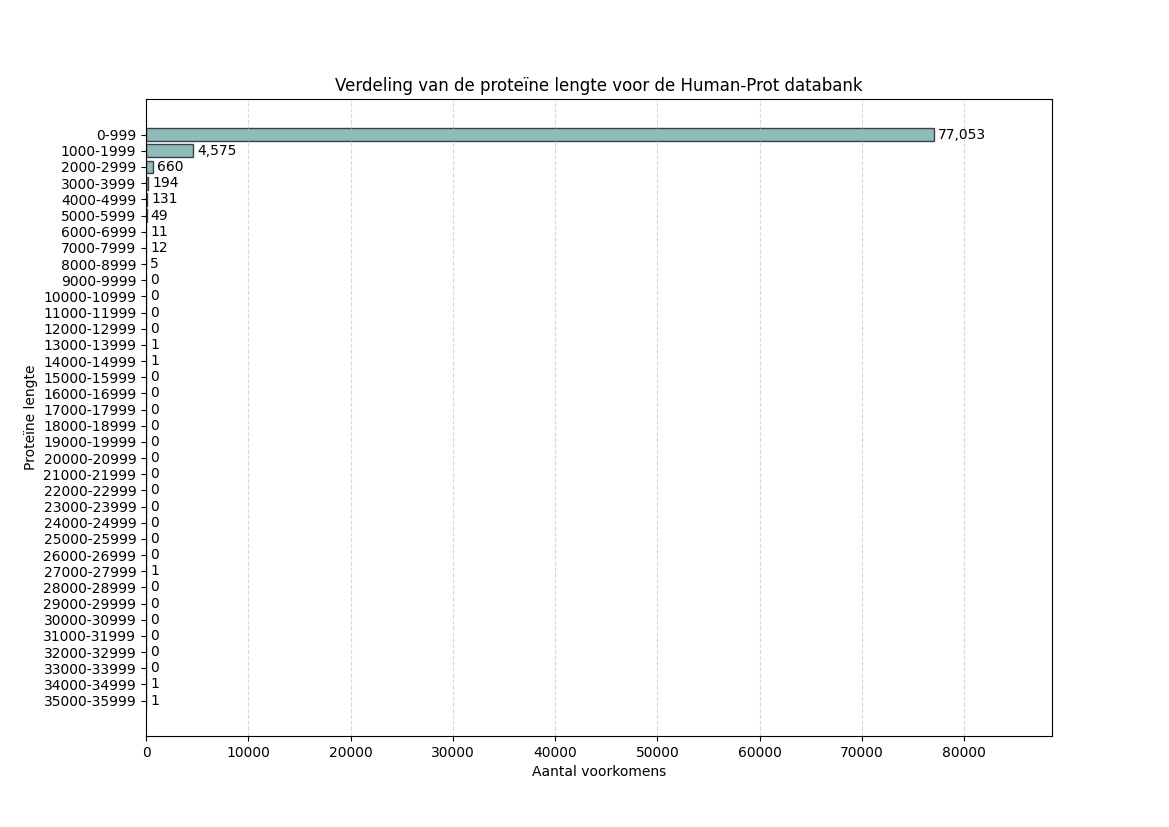
\includegraphics[width=0.5\linewidth]{humanprot_length_distribution_large}}
        \subfloat[Ingezoomd beeld van de lengtedistributie tot 1000 aminozuren lang]{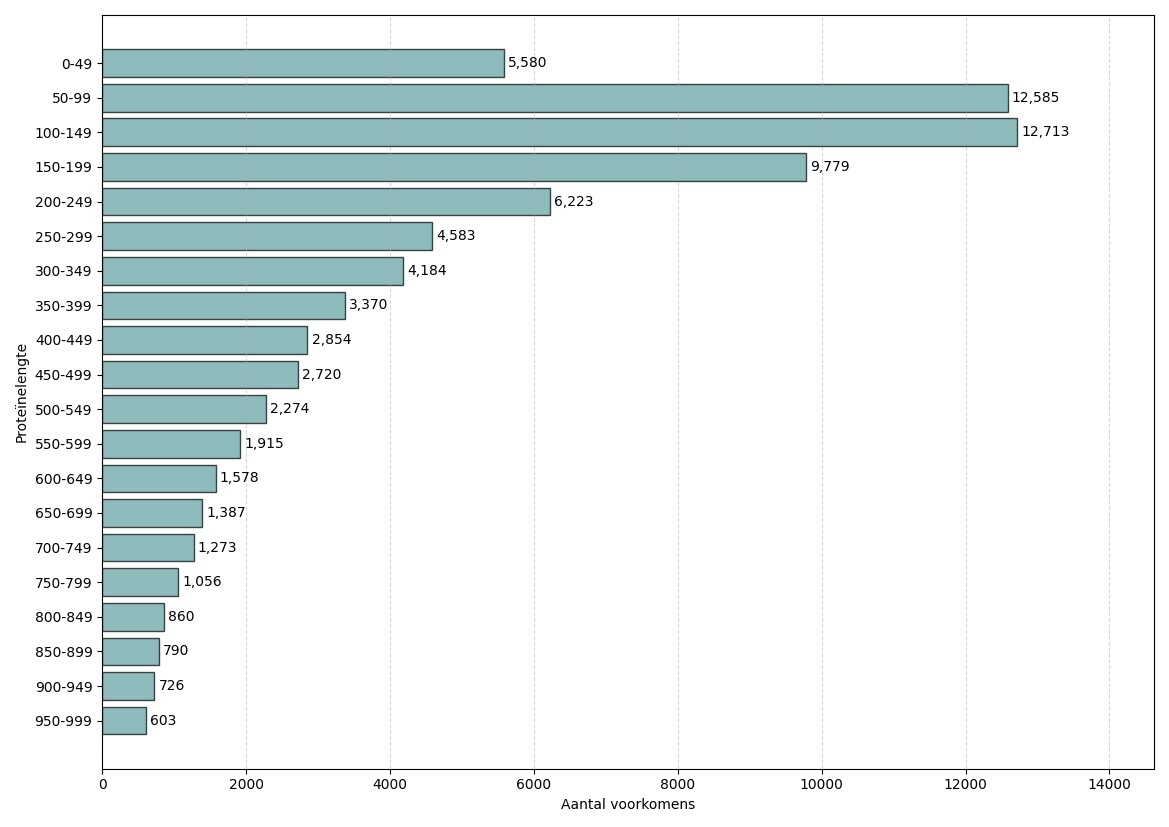
\includegraphics[width=0.5\linewidth]{humanprot_length_distribution_small}}
        \caption{Lengtedistributie van de proteïnen in de Human-Prot databank}\label{fig:humanprot_length}
    \end{figure}

    Enkele belangrijke conclusies dat we hier al uit kunnen trekken zijn dat dat zo goed als alle letters gebruikt worden (ook al zijn er maar 20 aminozuren).
    Dit komt doordat sommige letters eigenlijk een soort wildcard voorstellen.
    Zo staat ``X'' voor elk mogelijk aminozuur, ``Z'' voor ``Q'' of ``E'',\ldots

    Een tweede conclusie is dat de verdeling van de lengtes in de Swiss-Prot en Human-Prot datasets vergelijkbaar zijn.
    Het zwaartepunt van het aantal voorkomens ligt bij Swiss-Prot wel iets later (rond 100 vs rond 200).

    \subsection{Peptide zoekbestanden}\label{subsec:peptide-zoek-bestanden}
    Natuurlijk is een erg belangrijk deel van het opbouwen van een indexstructuur de zoek performantie achteraf.
    Hiervoor hebben we bij elke proteïnen databank een lijst aan peptiden die we proberen te zoeken.
    Voor onze beide databanken zijn enkele datasets opgesteld.

    \subsubsection{Swiss-prot} Voor deze databank hebben we enkele zoekbestanden voorzien.
    2 bestanden die gesampled zijn en een reeks aan effectieve zoekbestanden die een real-world scenario voorstellen.
    De 2 gesamplede bestanden zijn zo gekozen dat 1 ervan enkel tryptische peptiden bevat, terwijl de andere ook peptiden bevat met \textit{missed cleavage}.
    De eerste kan dus op dit moment al efficiënt door Unipept behandeld worden, terwijl dit voor de 2e niet kan.

    \paragraph{Sampled}
    Een kort overzicht van enkele statistieken over de gesamplede bestanden valt te zien in respectievelijk tabel~\ref{tab:swiss_geen_missed_cleavage} en tabel~\ref{tab:swiss_missed_cleavage}.

    \begin{table}[!h]
        \begin{minipage}{.5\linewidth}
            \centering
            \begin{tabular}{c c}
                Metriek                    & Waarde    \\
                \hline\hline
                Totaal aantal sequenties   & 100 000   \\
                Totale lengte              & 1 605 909 \\
                Minimale proteïne lengte   & 5         \\
                Maximale proteïne lengte   & 50        \\
                Gemiddelde proteïne lengte & 16.06     \\
                Mediaan proteïne lengte    & 13        \\
                Aantal vindbare peptiden   & 67 375    \\
                \hline
            \end{tabular}
            \caption{Eigenschappen van \newline het Swiss-Prot zoekbestand \newline zonder \textit{missed cleavage}}
            \label{tab:swiss_geen_missed_cleavage}
        \end{minipage}
        \begin{minipage}{.5\linewidth}
            \centering
            \begin{tabular}{ c c }
                Metriek                    & Waarde    \\
                \hline\hline
                Totaal aantal sequenties   & 100 000   \\
                Totale lengte              & 2 544 356 \\
                Minimale proteïne lengte   & 5         \\
                Maximale proteïne lengte   & 93        \\
                Gemiddelde proteïne lengte & 25.44     \\
                Mediaan proteïne lengte    & 23        \\
                Aantal vindbare peptiden   & 62 581    \\
                \hline
            \end{tabular}
            \caption{Eigenschappen van \newline het Swiss-Prot zoekbestand \newline met \textit{missed cleavage}}
            \label{tab:swiss_missed_cleavage}
        \end{minipage}
    \end{table}

    \paragraph{Real-life stalen}
    Om een beter beeld te krijgen over de performantie worden ook enkele real-life stalen uit een kleine micro-organisme gemeenschap gebruikt.
    Namelijk uit SIHUMIx\footnote{SImplified HUMan Intestinal microbiota}\cite{SIHUMI_first_introduction, SIHUMI_frequently_used}.
    Opnieuw wordt een overzicht van enkele eigenschappen gegeven in de volgende tabel.
    Elke \texttt{S<XX>} kolom stelt de waarden voor staal met bestandsnaam \texttt{S<XX>.txt} voor.
    Tijdens testen zullen deze zoekbestanden gebruikt worden in combinatie met de Swiss-Prot databank.

    \begin{table}[h!]
        \centering
        \begin{tabular}{ c c c c c c c }
            Metriek                    & S03     & S05     & S07     & S08     & S11     & S14     \\
            \hline\hline
            Totaal aantal sequenties   & 25 000  & 25 000  & 24 424  & 25 000  & 25 000  & 25 000  \\
            Totale lengte              & 420 544 & 420 423 & 373 633 & 316 114 & 366 922 & 430 674 \\
            Minimale proteïne lengte   & 6       & 6       & 6       & 6       & 6       & 6       \\
            Maximale proteïne lengte   & 50      & 50      & 47      & 43      & 50      & 50      \\
            Gemiddelde proteïne lengte & 16.82   & 16.82   & 15.30   & 12.64   & 14.68   & 17.23   \\
            Mediaan proteïne lengte    & 15      & 16      & 14      & 12      & 14      & 16      \\
            Aantal vindbare peptiden   & 2570    & 2698    & 3652    & 4135    & 3792    & 2761    \\
            \hline
        \end{tabular}
        \caption{Eigenschappen van de SIHUMIx zoekbestanden}
        \label{tab:sihumi_zoekbestanden}
    \end{table}

    \paragraph{Human-Prot} Voor deze databank hebben we 1 zoekbestand voorzien.
    Dit bestand bevat niet-tryptische peptiden, waardoor het dus op dit moment niet te zoeken valt in Unipept.
    Aangezien de dataset waarbij dit zoekbestand hoort zelf samengesteld is, hebben we ook zelf willekeurige samples genomen om een zoekbestand op te stellen.
    Hierdoor is elk van de peptiden die we zullen proberen te vinden effectief vindbaar in de dataset.
    Een kort overzicht van enkele eigenschappen is terug te vinden in tabel~\ref{tab:humanprot_zoekbestand}

    \begin{table}[h!]
        \centering
        \begin{tabular}{ c c }
            Metriek                    & Waarde        \\
            \hline\hline
            Totaal aantal sequenties   & 250000        \\
            Totale lengte              & 2 458 834 046 \\
            Minimale proteïne lengte   & 1             \\
            Maximale proteïne lengte & 12
            \\
            Gemiddelde proteïne lengte & 9.84          \\
            Mediaan proteïne lengte    & 10            \\
            Aantal vindbare peptiden   & 250000        \\
            \hline
        \end{tabular}
        \caption{Eigenschappen van het Human-Prot zoekbestand}
        \label{tab:humanprot_zoekbestand}
    \end{table}


% =====================================================================
% End matter
% =====================================================================

% ------------ REFERENCES ------------
    \printbibliography[heading=bibintoc,title={Referenties}] % check if bibliography is in table of contents


% ------------ APPENDIX ------------
    \appendix


    \section{Appendix: Your first appendix}
    Insert some figure or table here.

    \newpage


    \section{Appendix: Your second appendix}
    The second appendix was forced to start on a new page.

\end{document}